\documentclass[12pt]{article}
\usepackage[utf8]{inputenc}
\usepackage[T1]{fontenc}
\usepackage[polish]{babel}
\usepackage{amsmath}
\usepackage{amsthm}
\usepackage[margin=0.7in]{geometry}
\usepackage{dsfont}
\usepackage{mdframed}
\usepackage[many]{tcolorbox}
\usepackage{listings}
\usepackage[bottom]{footmisc}
% \usepackage{cite}
\usepackage{float}
\usepackage{graphicx}

\tcbuselibrary{theorems}

\newtcbtheorem[]{theo}{Twierdzenie}%
{
    breakable,
    colback=gray!5,
    colframe=gray!35!black,
    fonttitle=\bfseries,
    before skip=20 pt, 
    after skip=20pt
}{th}

\newtcbtheorem[]{defn}{Definicja}%
{
    breakable,
    colback=gray!5,
    colframe=gray!35!black,
    fonttitle=\bfseries,
    before skip=20 pt, 
    after skip=20pt
}{df}

\newtcbtheorem[]{prog}{Program}%
{
    breakable,
    colback=gray!5,
    colframe=gray!35!black,
    fonttitle=\bfseries,
    before skip=20 pt, 
    after skip=20pt
}{pr}

\lstdefinelanguage{Julia}%
{
    morekeywords={%
        exit,whos,edit,load,is,isa,isequal,typeof,tuple,ntuple,uid,hash,finalizer,convert,promote,%
        subtype,typemin,typemax,realmin,realmax,sizeof,eps,promote_type,method_exists,applicable,%
        invoke,dlopen,dlsym,system,error,throw,assert,new,Inf,Nan,pi,im,begin,while,for,in,return,%
        break,continue,macro,quote,let,if,elseif,else,try,catch,end,bitstype,ccall,do,using,module,%
        import,export,importall,baremodule,immutable,local,global,const,Bool,Int,Int8,Int16,Int32,%
        Int64,Uint,Uint8,Uint16,Uint32,Uint64,Float32,Float64,Complex64,Complex128,Any,Nothing,None,%
        function,type,typealias,abstract%
  },%
  sensitive=true,%
  morecomment=[l]\#,%
  morecomment=[n]{\#=}{=\#},%
  morestring=[s]{"}{"},%
  morestring=[m]{'}{'},%
}[keywords, comments, strings]%

\lstset{%
    language         = Julia,
    basicstyle       = \ttfamily,
    keywordstyle     = \bfseries\color{blue},
    columns          = fullflexible,
    stringstyle      = \color{magenta},
    commentstyle     = \color{gray},
    showstringspaces = false,
    numbers          = left,
    xleftmargin      = 2em
}

\title{\huge Metoda iteracyjna Müllera}
\date{Analiza Numeryczna (M) - Zadanie P2.4\\ \today}
\author{\Large Jakub Grobelny}

\begin{document}
\begin{titlepage}
\maketitle
\thispagestyle{empty}

\begin{abstract}
    Rozwiązywanie równań nielinowych jest jednym z podstawowych zagadnień analizy
    numerycznej. Polega ono na znajdowaniu miejsc zerowych funkcji, które nie są
    funkcjami liniowymi. Zostało opracowanych wiele metod iteracyjnych, które
    pozwalają znajdywać te miejsca. Niniejsze sprawozdanie jest podsumowaniem
    eksperymentu polegającego na porównaniu metody Müllera z innymi metodami 
    iteracyjnymi, a dokładniej z metodą siecznych oraz metodą Newtona.
\end{abstract}

\end{titlepage}

\newpage
\tableofcontents
\newpage

\section{Metoda iteracyjna Müllera}

Niech $p_n$ będzie wielomianem drugiego stopnia interpolującym funkcję $f$ w
punktach $x_{n-2},\, x_{n-1},\, x_n$. Zdefiniujmy $x_{n+1}$ jako miejsce zerowe
wielomianu $f$, które jest najbliższe $x_n$. Skoro wielomian $p_n$ interpoluje
funkcję $f$, to możemy oczekiwać, że jego miejsce zerowe znajdzie się relatywnie
blisko miejsca zerowego funkcji $f$. Można zauważyć, że w rzeczywistości ciąg 
miejsc zerowych kolejnych wielomianów interpolujących stanowi ciąg kolejnych
przybliżeń takiej wartości $\alpha$, że $f(\alpha) = 0$.

\begin{figure}[H]
    \centering
    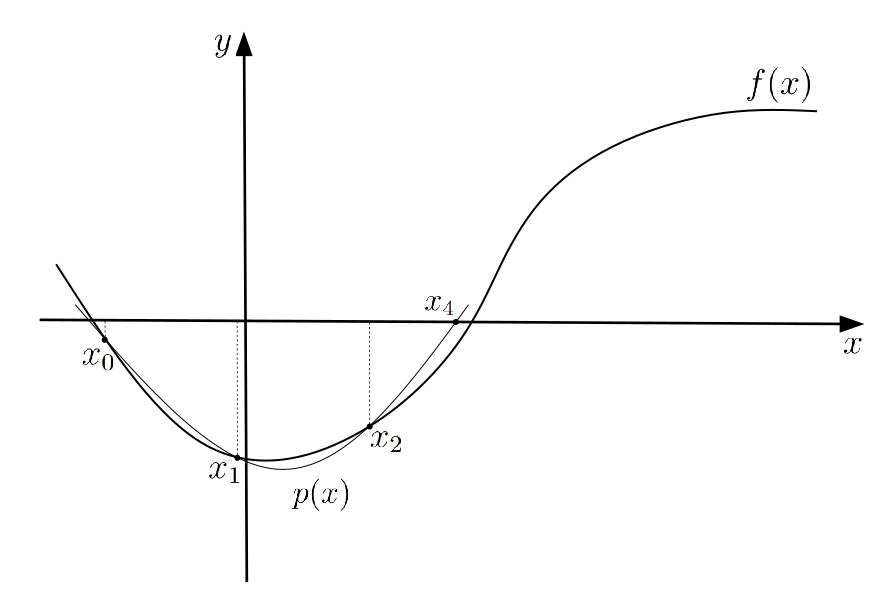
\includegraphics[scale=0.55]{plot_muller.png}
\caption{Graficzna interpretacja metody Müllera}
\label{figure:fig0}
\end{figure}

Na podstawie powyższej intuicji można wyprowadzić wzór na metodę iteracyjną,
działającą w opisany sposób.

\begin{defn}{Iloraz różnicowy \cite{kincaid}}{diffquot}
    Ilorazem różnicowym $n$-tego rzędu funkcji $f: X \to Y$ w punktach
    $x_0, x_1, ...,\,x_n$ nazywamy funkcję
    \[f[x_0, x_1, ...,\, x_n] := \sum_{i=0}^n\frac{f(x_i)}
    {\prod\limits_{\substack{{j=0}\\{j\neq i}}}{(x_i - x_j)}}\]
\end{defn}

\begin{defn}{Postać Newtona wielomianu interpolującego \cite{kincaid}}{polynewton}
    Mając funkcję $f$ oraz zadane $n+1$ punktów $x_0, x_1, ...,\,x_n$ można
    skonstruować wielomian $L_n$ stopnia $n$ interpolujący funkcję $f$ przy 
    użyciu następującego wzoru:
    \[L_n(x) := \sum_{i=0}^n{b_i\,p_i(x)},\]
    gdzie wielomiany $p_i$ dla $i = 0, 1, ...,\,n$ mają postać
    \[p_i(x) := \prod_{j=0}^{i-1}{(x-x_j)},\]
    zaś współcznniki $b_i$ definiujemy następująco:
    \[b_i := f[x_0, ...,\,x_i].\]
\end{defn}

Korzystając z definicji \ref{df:polynewton} możemy zapisać wielomian $p_n$ w
następującej postaci:
\[p_n(x) = f(x_n) + f[x_n, x_{n-1}](x-x_n) 
+ f[x_n, x_{n-1}, x_{n-2}](x-x_{n})(x-x_{n-1}),\]
którą dalej możemy przekształcić do
\[p_n(x) = f(x_n) +  \lambda(x-x_n) + f[x_n, x_{n-1}, x_{n-2}](x-x_n)^2,\]
gdzie
\[\lambda = f[x_n,x_{n-1}] + f[x_n, x_{n-2}] - f[x_{n-1}, x_{n-2}].\]

Mając wzór na wielomian $p_n$ można wyprowadzić wzór na jego miejsca zerowe, 
korzystając ze wzoru
\[x = \frac{-2c}{b \pm \sqrt{b^2 - 4ac}}\]
na miejsca zerowe funkcji $y = ax^2 + bx + c$.

Po podstawieniu otrzymujemy ostateczny wzór
\[x_{n+1} = x_n - 
\frac{2f(x_n)}
{\lambda \pm \sqrt{\lambda^2 -4f(x_n)f[x_n, x_{n-1}, x_{n-2}]}},
\label{mullerformula} \tag{1}\]
gdzie znak w mianowniku wybieramy tak, żeby wartość bezwzględna z mianownika
była możliwie największa. Dzięki temu uzyskamy to miejsce zerowe, które jest
położone najbliżej $x_n$.\newpage
Metoda Müllera jest metodą o złożoności w przybliżeniu równej 1.84.

Korzystając ze wzoru (\ref{mullerformula}) możemy napisać funkcję w języku
Julia, która będzie obliczać kolejne przybliżenie miejsca zerowego dla danych
dotychczasowych przybliżeń.

\begin{prog}{Implementacja metody Müllera}{progmuller}
\begin{lstlisting}
function mullers_method(x0, x1, x2, f)
    f0 = f(x0)
    f1 = f(x1)
    f2 = f(x2)

    numerator = BigFloat(2) * f2

    # Funkcja difference_quotient() oblicza iloraz roznicowy dla
    # zadanych punktow w postaci (x,y)
    lambda = difference_quotient([(x2, f2), (x1, f1)]) +
              difference_quotient([(x2, f2), (x0, f0)]) -
              difference_quotient([(x1, f1), (x0, f0)])
    
    x0_x1_x2_diff_quot = difference_quotient([
        (x0, f0), 
        (x1, f1), 
        (x2, f2)
    ])
    
    denom_r = sqrt(lambda^2.0 - 4.0*f(x2) * x0_x1_x2_diff_quot + 0im)
    denom_0 = lambda - denom_r
    denom_1 = lambda + denom_r

    denominator = abs(denom_0) > abs(denom_1) ? denom_0 : denom_1

    return x2 - numerator/denominator
end
\end{lstlisting}
\end{prog}

\section{Inne metody rozwiązywania równań nieliniowych}

\subsection{Metoda Newtona \cite{kincaid}}

Niech $f(x)$ będzie funkcją, której miejsce zerowe chcemy wyznaczyć numerycznie,
oraz niech $f(\alpha)=0$ i niech $x$ będzie przybliżeniem $\alpha$. Jeżeli
istnieje $f''$, to ze wzoru Taylora mamy
\[0 = f(\alpha) = f(x+h) = f(x) + hf'(x) + \mathcal{O}(h^2),\]
gdzie $h = \alpha - x$. Jeżeli $h$ dąży do zera, to możemy pominąć składnik
$\mathcal{O}(h^2)$. Mamy wtedy
\[0 = f(x) + hf'(x)\]
\[-f(x) = hf'(x)\]
\[h = \frac{-f(x)}{f'(x)}.\]
Przyjęliśmy, że $x$ jest przybliżeniem $\alpha$, więc 
\large$x-\frac{f(x)}{f'(x)}$\normalsize\, powinno być lepszym przybliżeniem.
Dzięki czemu możemy wyprowadzić wzór rekurencyjny na $n$-te przybliżenie:
\[x_n := x_{n-1} - \frac{f(x_{n-1})}{f'(x_{n-1})}.\label{newtonformula}\tag{2}\]

Metoda Newtona wymaga podania początkowego punktu $x_0$. Wybór tego punktu jest
istotny, gdyż metoda Newtona nie zawsze jest zbieżna.
Rząd zbieżności metody Newtona to 2 (zbieżność kwadratowa) z wyjątkiem
przypadków, gdy istnieją wielokrotne miejsca zerowe. Wtedy zbieżność jest
linowa (rząd zbieżności równy 1).

\begin{figure}[H]
    \centering
    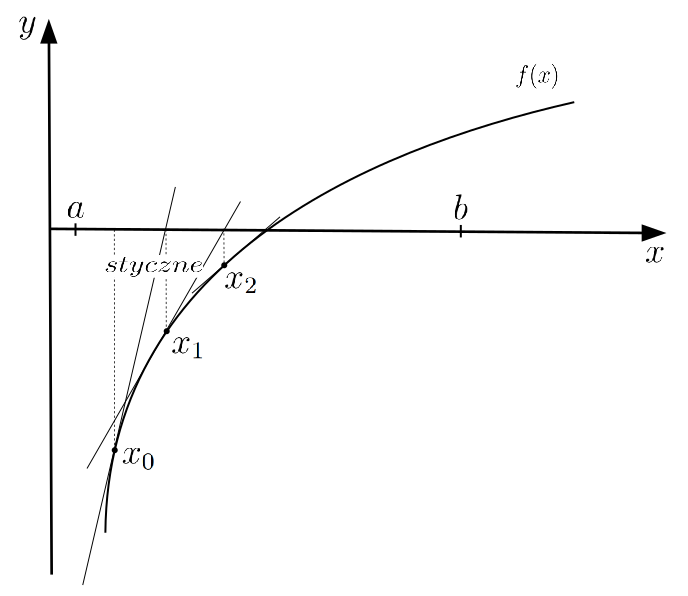
\includegraphics[scale=0.7]{plot_newton.png}
\caption{Graficzna interpretacja metody Newtona}
\label{figure:fig1}
\end{figure}

Obliczanie kolejnych przybliżeń w rzeczywistości polega na wyznaczaniu stycznej
do wykresu $f(x)$ w punkcie $x_n$, a następnie znajdowaniu punktu, w którym ta
styczna przecina oś $OX$. Otrzymany punkt przyjmujemy jako kolejne przybliżenie
$x_{n+1}$.\newpage

Implementacja metody Newtona w jęzku Julia przy użyciu wzoru 
(\ref{newtonformula}) jest bardzo prosta:

\begin{prog}{Implementacja metody Newtona}{prognewton}
\begin{lstlisting}
function newtons_method(x0, f, df)
    return x0 - f(x0) / df(x0)
end
\end{lstlisting}
\end{prog}

\subsection{Metoda siecznych \cite{kincaid}}

Wadą metody Newtona jest to, że trzeba znać pochodną funkcji $f(x)$, której
miejsce zerowe chcemy wyznaczyć.

Korzystając z faktu, że
\[f'(x_n) \approx \frac{f(x_n)-f(x_{n-1})}{x_n - x_{n-1}} = f[x_{n-1}, x_n],\]
możemy zastąpić pochodną we wzorze z metody Newtona na iloraz różnicowy, co daje
nam wzór
\[x_n:=x_{n-1} - f(x_{n-1})\frac{x_{n-1} - x_{n-2}}{f(x_{n-1}) - f(x_{n-2})}.\]

Rząd zbieżności metody siecznych to $\varphi = \frac{1+\sqrt{5}}{2} 
\approx 1.618$.

\begin{prog}{Implementacja metody siecznych}{secantprog}
\begin{lstlisting}
function secant_method(x0, x1, f)
    f0 = f(x0)
    f1 = f(x1)
    return x1 - f1 * (x1 - x0) / (f1 - f0)
end    
\end{lstlisting}
\end{prog}

Interpretacja graficzna metody siecznych jest taka, iż prowadzimy prostą
przechodzącą przez punkty $(x_{n-1}, f(x_{n-1}))$ oraz $(x_n, f(x_n))$, gdzie
$x_n$ i $x_{n-1}$ są poprzednimi przybliżeniami miejsca zerowego funkcji $f$, a 
następnie szukamy miejsca, w którym poprowadzona prosta przecina oś $OX$ i 
przyjmujemy to miejsce jako nowe przybliżenie $x_{n+1}$.

\begin{figure}[H]
    \centering
    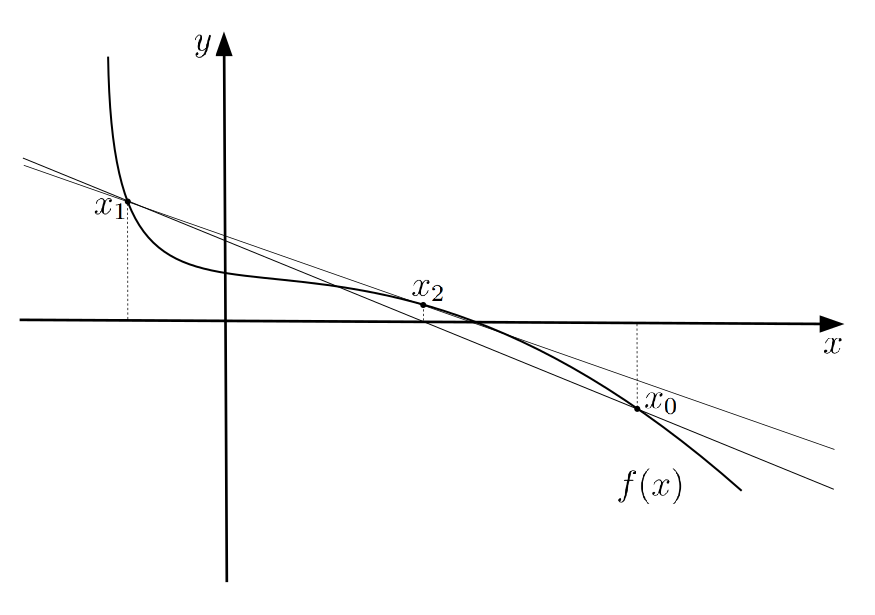
\includegraphics[scale=0.55]{plot_secant.png}
\caption{Graficzna interpretacja metody siecznych}
\label{figure:fig2}
\end{figure}

\section{Opis eksperymentu}

Celem niniejszego sprawozdania było sprawdzenie, jak metoda Müllera wypada na
tle innych metod rozwiązywania równań nieliniowych. W tym celu wszystkie trzy
metody zostały użyte do znalezienia miejsc zerowych różnych funkcji, a następnie
obliczona została liczba poprawnych cyfr w kolejnych iteracjach przy użyciu 
wzoru
\[\lfloor-log_{10}(\delta)\rfloor,\]
gdzie $\delta$ oznacza błąd względny otrzymanego wyniku.

Obliczenia zostały wykonane w języku Julia (wersja 1.0.1) przy użyciu 
256-bitowej precyzji (\texttt{setprecision(256)}).\newline

Metody były testowane w następujący sposób:
\begin{enumerate}
    \item Dla każdej funkcji wybrane zostało pierwsze przybliżenie $x_0$.
    \item Jednokrotnie wykonywano iterację metody Newtona aby uzyskać $x_1$.
    \item Jednokrotnie wykonywano iterację metody siecznych dla $x_0$ i $x_1$,
            uzyskując jako wynik $x_2$.
    \item Uruchamiano metodę Newtona dla $x_0$, metodę siecznych dla $x_0$ 
            i $x_1$ oraz metodę Müllera dla $x_0, x_1$ i $x_2$.
\end{enumerate}

Wybrany sposób daje delikatną przewagę metodzie siecznych oraz metodzie
Müllera, lecz pozwala zautomatyzować wybór wielu punktów początkowych. Biorąc
pod uwagę kwadratową zbieżność metody Newtona, nie powinno to znacząco
wpłynąć na wiarygodność pomiarów.

\section{Wyniki eksperymentu}

Uwaga: w tablicach z wynikami symbol $x^*$ oznacza, że obliczona została
dokładna wartość miejsca zerowego.

\subsection{$f(x) = x^2 - 3x + 2$}

\[f(x) = x^2 - 3x + 2\]
\[f'(x) = 2x - 3\]
\[x_0 = -0.2\]
\begin{center}
    Dokładna wartość miejsca zerowego: $x = 1$
\end{center}

\begin{table}[H]
\centering
\begin{tabular}{|c|c|c|c|}
    \hline
    $n$ & Newton & Sieczne & Müller  \\ \hline\hline
    0  & 0.0     & 0.0     & 0.0     \\ \hline
    1  & 0.0     & 0.0     & 0.0     \\ \hline
    2  & 1.0     & 0.0     & 0.0     \\ \hline
    3  & 2.0     & 1.0     & 7.6e+01 \\ \hline
    4  & 4.0     & 2.0     & 7.6e+01 \\ \hline
    5  & 8.0     & 3.0     & $x^*$\\ \hline
    6  & 1.6e+01 & 5.0     & $x^*$\\ \hline
    7  & 3.3e+01 & 8.0     & $x^*$\\ \hline
    8  & 6.7e+01 & 1.4e+01 & $x^*$\\ \hline
    9  & 7.6e+01 & 2.3e+01 & $x^*$\\ \hline
    10 & 7.6e+01 & 3.7e+01 & $x^*$\\ \hline
    11 & 7.6e+01 & 6.1e+01 & $x^*$\\ \hline
    12 & 7.6e+01 & 7.6e+01 & $x^*$\\ \hline
    13 & 7.6e+01 & 7.6e+01 & $x^*$\\ \hline
    14 & 7.6e+01 & $x^*$   & $x^*$\\ \hline
    15 & 7.6e+01 & $x^*$   & $x^*$\\ \hline
    16 & 7.6e+01 & $x^*$   & $x^*$\\ \hline
    17 & 7.6e+01 & $x^*$   & $x^*$\\ \hline
    18 & 7.6e+01 & $x^*$   & $x^*$\\ \hline
    19 & 7.6e+01 & $x^*$   & $x^*$\\ \hline
    20 & 7.6e+01 & $x^*$   & $x^*$\\ \hline
\end{tabular}
\caption{Porównanie liczby poprawnych cyfr w kolejnych iteracjach metod}
\label{table:table1}
\end{table}

\begin{figure}[H]
    \centering
    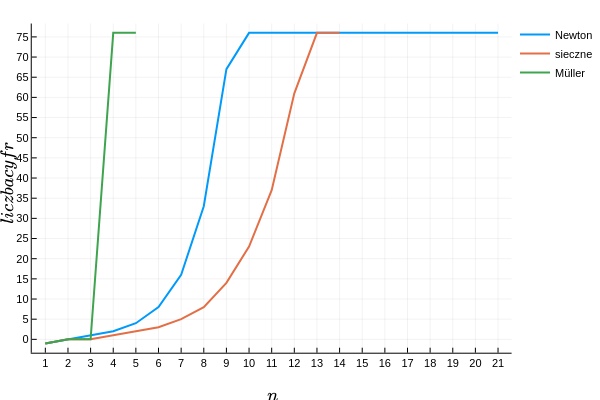
\includegraphics[scale=0.7]{plot1.png}
\caption{Szybkość zbieżności wszystkich metod do miejsca 
         zerowego $f(x) = x^2 - 3x + 2$}
\label{figure:plot1}
\end{figure}

W przypadku funkcji $f(x) = x^2 - 3x + 2$ można zaobserwować wyjątkową przewagę
metody Müllera nad metodą siecznych i metodą Newtona. Jest ona najprawdopodobniej
spowodowana tym, iż funkcja $f$ jest wielomianem stopnia drugiego, tak samo jak 
wielomian interpolujący $p_n$, który jest używany do obliczania kolejnych 
przybliżeń. Istnieje tylko jeden wielomian stopnia drugiego przechodzący przez
dane trzy punkty, a więc $p_n \equiv f$.

\subsection{$f(x) = \sqrt{x} - 4$}

\[f(x) = \sqrt{x} - 4\]
\[f'(x) = \frac{1}{2}x\]
\[x_0 = 18\]
\begin{center}
    Dokładna wartość miejsca zerowego: $x = 16$
\end{center}

\begin{table}[H]
\centering
\begin{tabular}{|c|c|c|c|}
    \hline
    $n$ & Newton & Sieczne & Müller   \\ \hline\hline
    0  & 0.0     & 0.0     &  0.0     \\ \hline
    1  & 2.0     & 2.0     &  2.0     \\ \hline
    2  & 5.0     & 3.0     &  3.0     \\ \hline
    3  & 1.1e+01 & 6.0     &  8.0     \\ \hline
    4  & 2.3e+01 & 1.1e+01 &  1.5e+01 \\ \hline
    5  & 4.7e+01 & 1.9e+01 &  2.8e+01 \\ \hline
    6  & $x^*$   & 3.1e+01 &  5.3e+01 \\ \hline
    7  & $x^*$   & 5.1e+01 &  $x^*$   \\ \hline
    8  & $x^*$   & $x^*$   &  $x^*$   \\ \hline
\end{tabular}
\caption{Porównanie liczby poprawnych cyfr w kolejnych iteracjach metod}
\label{table:table2}
\end{table}
    
\begin{figure}[H]
    \centering
    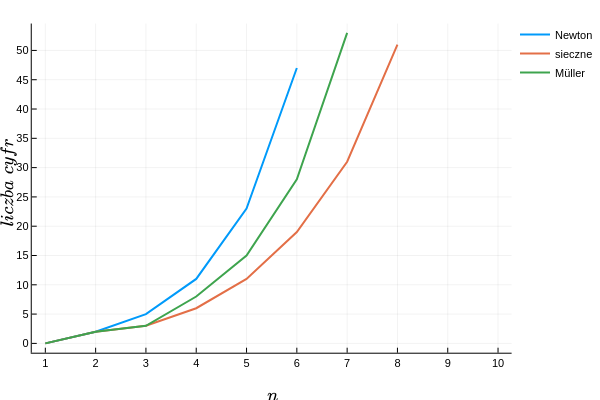
\includegraphics[scale=0.7]{plot2.png}
\caption{Szybkość zbieżności wszystkich metod do miejsca 
            zerowego $f(x) = \sqrt{x} - 4$}
\label{figure:plot2}
\end{figure}

\subsection{$f(x) = 2(x-1)(x-2)(x-1.5)(x-4)$}

\[f(x) = 2(x-1)(x-2)(x-1.5)(x-4)\]
\[f'(x) = 8(x^3 - 6.375x^2 + 12.25x - 7.25)\]
\[x_0 = 3\]
\begin{center}
    Dokładna wartość miejsca zerowego: $x = 2$
\end{center}

\begin{table}[H]
\centering
\begin{tabular}{|c|c|c|c|}
    \hline
    $n$ & Newton & Sieczne & Müller  \\ \hline\hline
    0  & 0.0     & 0.0     & 0.0     \\ \hline
    1  & 1.0     & 1.0     & 1.0     \\ \hline
    2  & 1.0     & 1.0     & 1.0     \\ \hline
    3  & 2.0     & 2.0     & 2.0     \\ \hline
    4  & 5.0     & 2.0     & 4.0     \\ \hline
    5  & 9.0     & 4.0     & 8.0     \\ \hline
    6  & 1.9e+01 & 6.0     & 1.5e+01 \\ \hline
    7  & 3.7e+01 & 9.0     & 2.8e+01 \\ \hline
    8  & 7.4e+01 & 1.5e+01 & 5.2e+01 \\ \hline
    9  & $x^*$   & 2.4e+01 & $x^*$   \\ \hline
    10 & $x^*$   & 3.8e+01 & $x^*$   \\ \hline
    11 & $x^*$   & 6.1e+01 & $x^*$   \\ \hline
    12 & $x^*$   & $x^*$   & $x^*$   \\ \hline
    13 & $x^*$   & $x^*$   & $x^*$   \\ \hline
\end{tabular}
\caption{Porównanie liczby poprawnych cyfr w kolejnych iteracjach metod}
\label{table:table3}
\end{table}

\begin{figure}[H]
    \centering
    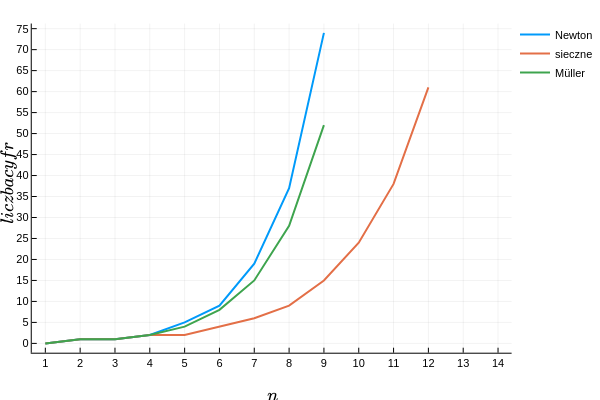
\includegraphics[scale=0.7]{plot3.png}
\caption{Szybkość zbieżności wszystkich metod do miejsca 
            zerowego $f(x) = 2(x-1)(x-2)(x-1.5)(x-4)$}
\label{figure:plot3}
\end{figure}

\subsection{$f(x) = x2^x -2$}

\[f(x) = x2^x -2\]
\[f'(x) = 2^x (x\,ln(2)+1)\]
\[x_0 = 0.123\]
\begin{center}
    Dokładna wartość miejsca zerowego: $x = 1$
\end{center}

\begin{table}[H]
\centering
\begin{tabular}{|c|c|c|c|}
    \hline
    $n$ & Newton & Sieczne & Müller  \\ \hline\hline
    0  & 0.0     & 0.0     & 0.0     \\ \hline
    1  & 0.0     & 0.0     & 0.0     \\ \hline
    2  & 0.0     & 0.0     & 0.0     \\ \hline
    3  & 1.0     & 0.0     & 1.0     \\ \hline
    4  & 3.0     & 1.0     & 2.0     \\ \hline
    5  & 7.0     & 2.0     & 5.0     \\ \hline
    6  & 1.5e+01 & 4.0     & 1.0e+01 \\ \hline
    7  & 3.0e+01 & 7.0     & 2.0e+01 \\ \hline
    8  & 4.7e+01 & 1.2e+01 & 3.7e+01 \\ \hline
    9  & 6.4e+01 & 2.0e+01 & 6.9e+01 \\ \hline
    10 & $x^*$   & 3.3e+01 & $x^*$   \\ \hline
    11 & $x^*$   & 5.4e+01 & $x^*$   \\ \hline
    12 & $x^*$   & $x^*$   & $x^*$   \\ \hline
\end{tabular}
\caption{Porównanie liczby poprawnych cyfr w kolejnych iteracjach metod}
\label{table:table4}
\end{table}

\begin{figure}[H]
    \centering
    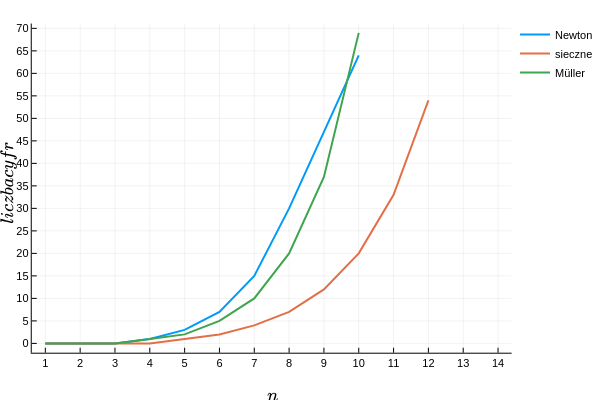
\includegraphics[scale=0.7]{plot4.png}
\caption{Szybkość zbieżności wszystkich metod do miejsca 
            zerowego $f(x) = x2^x -2$}
\label{figure:plot4}
\end{figure}

\subsection{$f(x) = ln|x|$}

\[f(x) = ln|x|\]
\[f'(x) = \frac{1}{x}\]
\[x_0 = \frac{1}{2}\]
\begin{center}
    Dokładna wartość miejsca zerowego: $x = 1$
\end{center}

\begin{table}[H]
\centering
\begin{tabular}{|c|c|c|c|}
    \hline
    $n$ & Newton & Sieczne & Müller     \\ \hline\hline
    0  &  0.0     &  0.0     &  0.0     \\ \hline
    1  &  0.0     &  0.0     &  0.0     \\ \hline
    2  &  1.0     &  1.0     &  1.0     \\ \hline
    3  &  4.0     &  2.0     &  2.0     \\ \hline
    4  &  8.0     &  4.0     &  5.0     \\ \hline
    5  &  1.7e+01 &  6.0     &  9.0     \\ \hline
    6  &  3.4e+01 &  1.1e+01 &  1.8e+01 \\ \hline
    7  &  7.0e+01 &  1.8e+01 &  3.3e+01 \\ \hline
    8  &  $x^*$   &  3.0e+01 &  6.1e+01 \\ \hline
    9  &  $x^*$   &  4.8e+01 &  $x^*$   \\ \hline
    10 &  $x^*$   &  $x^*$   &  $x^*$   \\ \hline
\end{tabular}
\caption{Porównanie liczby poprawnych cyfr w kolejnych iteracjach metod}
\label{table:table5}
\end{table}

\begin{figure}[H]
    \centering
    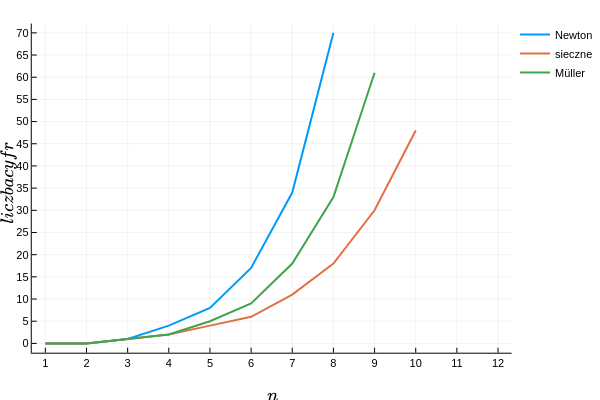
\includegraphics[scale=0.7]{plot5.png}
\caption{Szybkość zbieżności wszystkich metod do miejsca 
            zerowego $f(x) = ln|x|$}
\label{figure:plot5}
\end{figure}

\subsection{$f(x) = cos(xsinx)$}

\[f(x) = cos(xsinx)\]
\[f'(x) = sin(x\,sin(x))(-(sin(x)+x\,cos(x)))\]
\[x_0 = -1\]
\begin{center}
    Dokładna wartość miejsca zerowego: $x = -\frac{\pi}{2}$
\end{center}

\begin{table}[H]
\centering
\begin{tabular}{|c|c|c|c|}
    \hline
    $n$ & Newton & Sieczne & Müller  \\ \hline\hline
    0  & 0.0     & 0.0     & 0.0     \\ \hline
    1  & 1.0     & 1.0     & 1.0     \\ \hline
    2  & 2.0     & 2.0     & 2.0     \\ \hline
    3  & 4.0     & 3.0     & 3.0     \\ \hline
    4  & 9.0     & 5.0     & 6.0     \\ \hline
    5  & 1.6e+01 & 8.0     & 1.2e+01 \\ \hline
    6  & 1.6e+01 & 1.3e+01 & 1.6e+01 \\ \hline
    7  & 1.6e+01 & 1.6e+01 & 1.6e+01 \\ \hline
    8  & 1.6e+01 & 1.6e+01 & 1.6e+01 \\ \hline
    9  & 1.6e+01 & 1.6e+01 & 1.6e+01 \\ \hline
    10 & 1.6e+01 & 1.6e+01 & 1.6e+01 \\ \hline
    11 & 1.6e+01 & 1.6e+01 & 1.6e+01 \\ \hline
    \vdots & \vdots & \vdots & \vdots \\ \hline
\end{tabular}
\caption{Porównanie liczby poprawnych cyfr w kolejnych iteracjach metod}
\label{table:table6}
\end{table}

Można zauważyć, że w tym przypadku żadna z metod nie obliczyła dokładnej
wartości miejsca zerowego $-\frac{\pi}{2}$ i od pownego momentu przybliżenia
przestają się poprawiać (funkcje zwracały dokładnie ten sam wynik w kolejnych
iteracjach).

\begin{figure}[H]
    \centering
    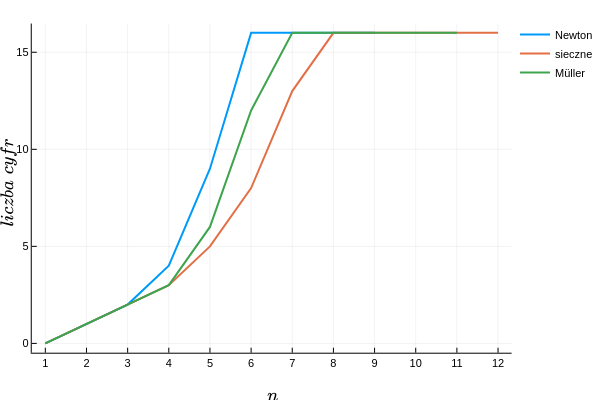
\includegraphics[scale=0.7]{plot6.png}
\caption{Szybkość zbieżności wszystkich metod do miejsca 
            zerowego $f(x) = cos(xsinx)$}
\label{figure:plot6}
\end{figure}

\section{Podsumowanie}

Zgodnie z oczekiwaniami, w niemal każdym przykładzie wyniki odzwierciedlają
złożoność każdej z metod. Metoda Müllera jest zbieżna szybciej niż metoda
siecznych, lecz jest deklasowana przez metodę Newtona, która ma zbieżność
kwadratową. Zdecydowaną zaletą metody Müllera jest fakt, iż nie musimy znać
wzoru na pochodną funkcji, której miejsce zerowe aproksymujemy. Metoda Müllera
okazała się skuteczniejsza jedynie w przypadku znajdowania pierwiastków
wielomianów drugiego stopnia (co jest oczywistą konsekwencją tego, iż jest ona
oparta o interpolację funkcji wielomianami stopnia drugiego).

Po przeprowadzeniu powyższych obliczeń, można również eksperymentalnie
wyznaczyć rząd zbieżności metody Müllera -- gdy podzielimy otrzymaną dokładność
przez tę, którą otrzymaliśmy jedną iterację wcześniej, otrzymany wynik będzie
oscylował w okolicy 1.84. 
Na przykład dla $f(x) = ln|x|$ mamy
\[\frac{9}{5} = 1.8\]
\[\frac{33}{18} \approx 1.833333333\]
\[\frac{611}{33} \approx 1.848484848.\]
Powyższe obliczenia można również zastosować dla metody Newtona:
\[\frac{8}{4} = 2\]
\[\frac{17}{8} = 2.125\]
\[\frac{34}{17} = 2,\]
oraz metody siecznych:
\[\frac{18}{11} \approx 1.636363636\]
\[\frac{30}{18} \approx 1.666666667\]
\[\frac{48}{30} = 1.6.\]
\newline

Podsumowując, metoda Müllera jest bez wątpienia przydatną metodą rozwiązywania
równań nielinowych, ze względu na to, iż jest stosunkowo szybka, oraz nie wymaga
znajomości pochodnej. Jest ona niestety nieco bardziej skomplikowana niż 
pozostałe dwie metody, oraz wymaga o wiele więcej obliczeń.

\addcontentsline{toc}{section}{Bibliografia}
\bibliography{bibliografia}{}
\bibliographystyle{plain}

\end{document}